

\savegeometry{beamergeo}
\begin{emptyframe}
\frametitle{Summary}
\centerline{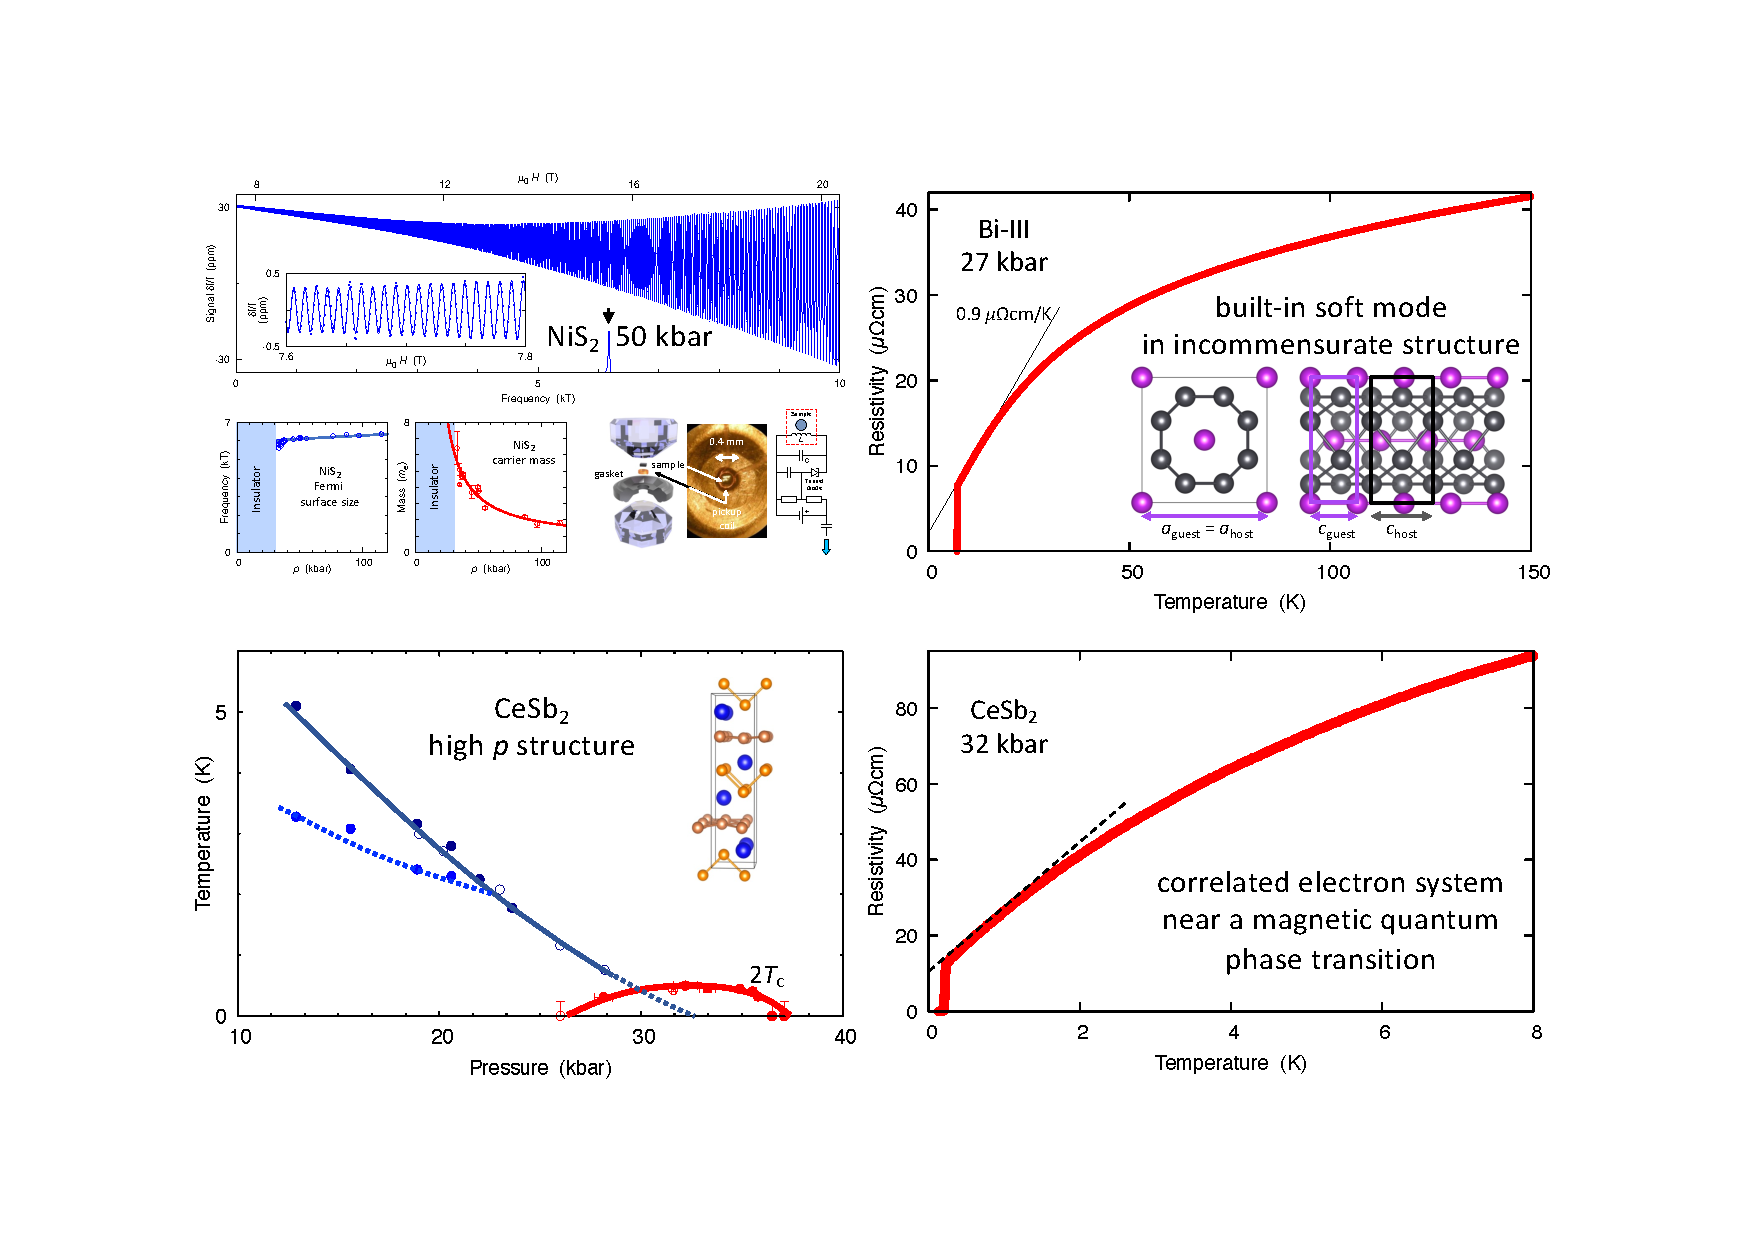
\includegraphics[width=\columnwidth]{EndingPicture3.pdf}}
%\vspace{-1em}
%\begin{center}
% Soft modes are built into some quasiperiodic structures. \\
%\mbox{\small QCP $\rightarrow$ superconductivity. Low-energy, (over)damped excitations $\rightarrow$ nFL transport}
\centerline{\small High-$p$ QO in Mott metal; non-Fermi liquid transport and superconductivity}

% \begin{itemize}
%   \item Fe-based superconductors YFe$_2$Ge$_2$ and LuFe$_2$Ge$_2$
%   \item Superconductivity in high-pressure CeSb$_2$, high $B_{c2}$
%   \item Integrated search loop for materials discovery
% \end{itemize}
% \vfill
% \centerline{\makebox[\linewidth]{\rule{0.85\textwidth}{0.4pt}}}

% \centerline{\scriptsize Squire PRL {\bf 131,} 026001 (2023)}


%\end{center}
% \vspace*{\fill}
% \centerline{\makebox[\linewidth]{\rule{0.85\textwidth}{0.4pt}}}
% \centerline{\scriptsize P. Brown Sci. Adv. (2018)}
\end{emptyframe}
%\restoregeometry
\loadgeometry{beamergeo}

%%% Local Variables: 
%%% mode: latex
%%% TeX-master: "GroTalk"
%%% End: 
